%%%% Paramétrage du cours %%%%
\def\xxactivite{Cours}
\def\xxauteur{\textsl{Xavier Pessoles}}

\fichetrue
\proftrue
\tdfalse
\coursfalse

\def\xxnumpartie{Rév -- Stat}
\def\xxpartie{Modélisation des actions mécaniques dans les systèmes}
\def\xxnumchapitre{ Révisions 2\vspace{.2cm}}
\def\xxchapitre{\hspace{.12cm} Modélisation du frottement}

\def\xxpied{%
Révision statique -- Modélisation des actions mécaniques\\
Fiche 2 -- \xxactivite%
}


\def\xxcompetences{%
\textsl{%
\textbf{Savoirs et compétences :}\\
%\begin{itemize}[label=\ding{112},font=\color{ocre}] 
%\item \textit{Res1.C2} : principe fondamental de la dynamique;
%\item \textit{Res1.C1.SF1} : proposer une démarche permettant la détermination de la loi de mouvement.
%\end{itemize}
}}


\iflivret
\input{../../style/new_pagegarde}
\else
\input{../../style/new_pagegarde}
\fi
\setlength{\columnseprule}{.1pt}

\vspace{2cm}
\pagestyle{fancy}
\thispagestyle{plain}


\section{Modélisation du contact ponctuel entre 2 pièces}
\subsection{Torseur des actions mécaniques}
\noindent\begin{minipage}[c]{.7\linewidth}
Considérons le contact ponctuel ponctuel entre deux pièces \textbf{1} et \textbf{2}. En considérant la liaison parfaite, le torseur des actions mécaniques de 1 sur 2 s'écrit sous la forme suivante : $\torseurstat{T}{1}{2}=\torseurl{F_{12} \vect{n_{12}}}{\vect{0}}{I}$ en notant $\vect{n_{12}}$ le vecteur normal au contact orienté de 1 vers 2. 
En considérant que la liaison n'est pas parfaite, plusieurs situation peuvent se présenter.  
\end{minipage}\hfill
\begin{minipage}[c]{.25\linewidth}
\begin{center}
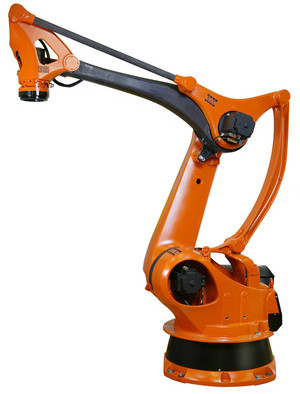
\includegraphics[width=\linewidth]{fig_01}
\end{center}
\end{minipage}

\begin{itemize}
\item Si on considère qu'un effort tend à faire translater 2 suivant $\vect{t_{12}}$, le torseur des actions mécaniques de 1 sur 2 peut alors s'écrire sous la forme $\torseurstat{T}{1}{2}=\torseurl{N_{12} \vect{n_{12}}+T_{12} \vect{t_{12}}}{\vect{0}}{I}$.
\item Si on considère qu'un effort tend à faire rouler 2 autour de $\vect{z_{12}}$, le torseur des actions mécaniques de 1 sur 2 peut alors s'écrire sous la forme $\torseurstat{T}{1}{2}=\torseurl{N_{12} \vect{n_{12}}}{M_{r12} \vect{z}}{I}$ avec $M_{r12}$ moment de résistance au roulement.
\item Si on considère qu'un effort tend à faire pivoter 2 autour de $\vect{n_{12}}$, le torseur des actions mécaniques de 1 sur 2 peut alors s'écrire sous la forme $\torseurstat{T}{1}{2}=\torseurl{N_{12} \vect{n_{12}}}{M_{p12} \vect{n_{12}}}{I}$ avec $M_{p12}$ moment de résistance au pivotement.
\end{itemize}

\begin{rem}
Il est possible de modéliser l'ensemble des composantes dues au frottement dans un même torseur. 

On fait l'hypothèse ici d'un problème plan, mais il peut aisément être adapté à un modèle 3D. 
\end{rem}

\subsection{Facteur de glissement et d'adhérence}
\noindent\begin{minipage}[c]{.7\linewidth}
Considérons la pièce 2 sur un plan incliné 1. Notons $\varphi_a$ l'angle à partir duquel la pièce 2 se met à glisser sur le plan. On appelle  $f_a=\tan\varphi_a$ le facteur d'adhérence.

On constate expérimentalement qu'une fois la pièce est en mouvement, si on diminue l'angle $\varphi$, la pièce continue à glisser, jusqu'à un angle  $\varphi_g$. On appelle \textbf{$f_g=\tan\varphi_g$} le facteur de glissement.
\end{minipage}\hfill
\begin{minipage}[c]{.25\linewidth}
\begin{center}
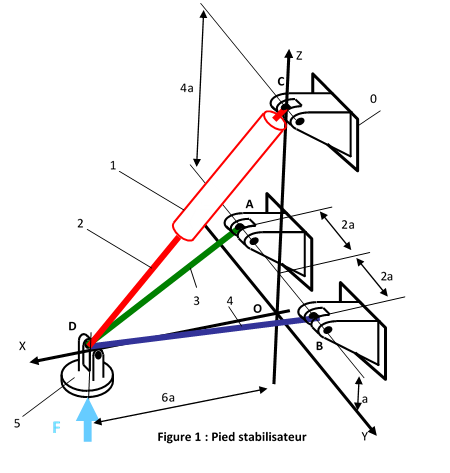
\includegraphics[width=\linewidth]{fig_02}
\end{center}
\end{minipage}

Ces facteurs sont sans unité. Ils dépendent de la nature des matériaux en contact ainsi que de la nature des surfaces de contact (et d'un lubrifiant éventuel). Ils sont indépendants de l'effort de 2 sur 1. Ces deux facteurs étant relativement proches, on fera l'hypothèse que $f=f_a=f_g$. 

\subsection{Modélisation de l'adhérence et du glissement -- Lois de Coulomb}

\noindent\begin{minipage}[t]{.35\linewidth}
\begin{center}
\textbf{Cas 1 -- Glissement -- $\vectv{I}{2}{1}\neq \vect{0}$}
\end{center}

\begin{itemize}
\item Connaissant le sens et la direction de $\vectv{I}{2}{1}$, alors $\vect{t_{12}}$ s'oppose à $\vectv{I}{2}{1}$.
\item $|T_{12}| = f |N_{12}|$.
\item La vecteur vitesse appartenant au plan tangent au contact, on dit que l'effort résultant ($\vect{F_{12}}=N_{12} \vect{n_{12}}+T_{12} \vect{t_{12}}$) est sur le cône de frottement. 
\end{itemize}
\end{minipage}\hfill
\begin{minipage}[t]{.35\linewidth}
\begin{center}
\textbf{Cas 2 -- Adhérence -- $\vectv{I}{2}{1} = \vect{0}$}
\end{center}

\begin{itemize}
\item La direction de $\vect{t_{12}}$ n'est pas connue. 
\item $|T_{12}| \leq f |N_{12}|$.
\item La direction $\vect{t_{12}}$ n'étant pas connue, on dit que l'effort résultant ($\vect{F_{12}}=N_{12} \vect{n_{12}}+T_{12} \vect{t_{12}}$) appartient au cône d'adhérence. 
\end{itemize}
\end{minipage}\hfill
\begin{minipage}[t]{.29\linewidth}
$\quad$
\begin{center}
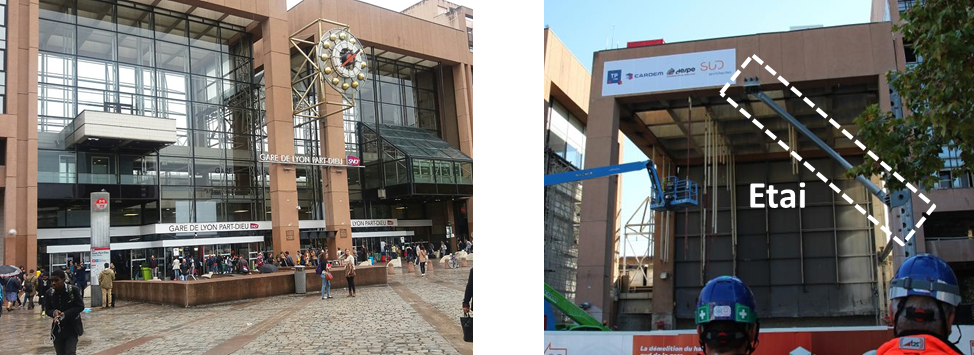
\includegraphics[width=\linewidth]{fig_03}
\end{center}
\end{minipage}

\begin{rem}
En considérant que la direction du vecteur vitesse peut décrire le plan tangent au contact, la résultante des efforts $\vect{F_{12}}$ décrit alors un cône. On parle donc de cône d'adhérence. 
\end{rem}

\subsection{Modélisation de la résistance au roulement et au pivotement}
\noindent\begin{minipage}[t]{.49\linewidth}
\begin{center}
\textbf{Modélisation de la résistance au roulement}
\end{center}
\begin{itemize}
\item Le moment de résistance au roulement $\vect{M_{r12}}$ s'oppose à $\vecto{2}{1}\cdot \vect{z}$. 
\item On note $r$ le coefficient de résistance au roulement ([m]) et on a $||\vect{M_{r12}}||=r||\vect{N_{12}} ||$.
\end{itemize}

\end{minipage}\hfill
\begin{minipage}[t]{.49\linewidth}
\begin{center}
\textbf{Modélisation de la résistance au pivotement}
\end{center}
\begin{itemize}
\item Le moment de résistance au pivotement $\vect{M_{p12}}$ s'oppose à $\vecto{2}{1}\cdot \vect{n_{12}}$. 
\item On note $p$ le coefficient de résistance au pivotement ([m]) et on a $||\vect{M_{p12}}||=p||\vect{N_{12}} ||$.
\end{itemize}
\end{minipage}

\vspace{1cm}

\noindent\begin{minipage}[t]{.69\linewidth}
Ainsi pour modéliser la résistance au roulement, on peut faire l'hypothèse que l'action normale de 1 sur 2 est <<~avancée~>> de $r$ par rapport au point $I$. 
\end{minipage}
\hfill
\begin{minipage}[t]{.29\linewidth}
$\quad$
\vspace{-.5cm}
\begin{center}
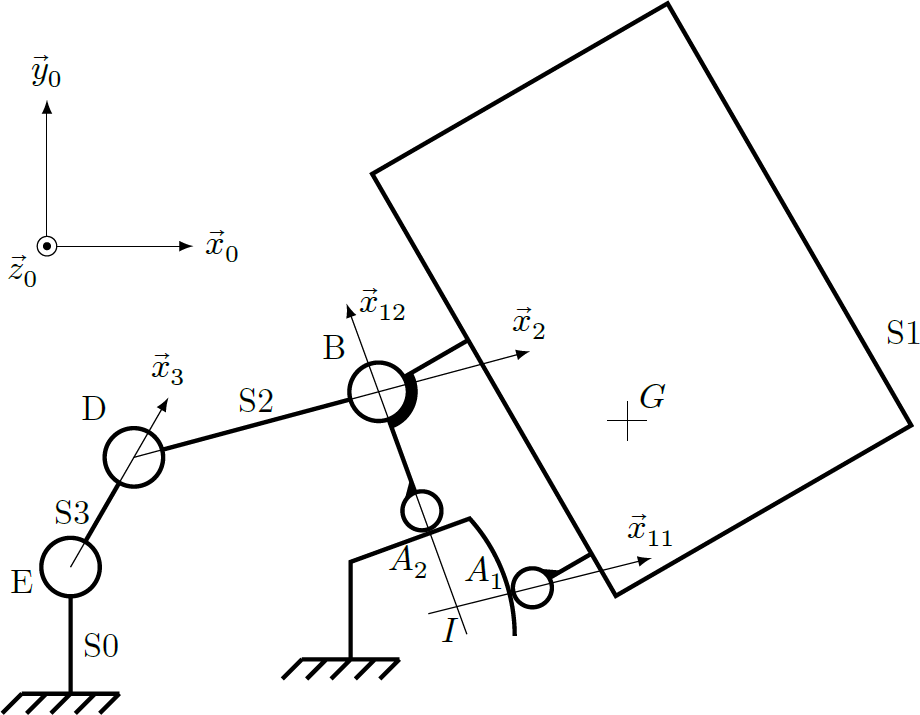
\includegraphics[width=\linewidth]{fig_04}
\end{center}
\end{minipage}

\section{Modélisation locale des actions mécaniques}
\begin{defi}
Localement, les actions mécaniques dans un contact ponctuel avec frottement peuvent être modélisées par le torseur suivant :
$
\torseurstat{T}{1}{2}=
\torseurl{%
\vect{R_{(1\rightarrow 2)}} 
= \iint\limits_{\mathcal{S}} f(M) \vect{u(M)} \text{d}\mathcal{S}}{%
\vectm{P}{1}{2} = \iint\limits_{\mathcal{S}}\vect{PM}\wedge \text{d}\vectf{1}{2}}{M}
$.

La densité surfacique d'effort peut alors se décomposer sur le vecteur normal au contact et sur un vecteur appartenant au plan tangent au contact. On a alors$f(M) \vect{u(M)} = p_{12}(M)\vect{n_{12}}+\vect{\tau_{12}}(M)$. 
Dans le cas du glissement : $||\vect{\tau_{12}}(M)||=p_{12}\cdot f$.
En notant : 
\begin{itemize}
\item $p_{12}(M)$ pression de contact au point $M$ (en $\left[\text{Nm}^{-2}\right]$);
\item $\vect{\tau_{12}}(M)$ : la projection tangentielle de la densité surfacique (norme en $\left[\text{Nm}^{-2}\right]$);
\item $f$ facteur de frottement.
\end{itemize}
\end{defi}

\section{Résolution des problèmes d'arc-boutement}
L'arc-boutement est un phénomène de blocage d'une liaison (souvent glissière ou pivot glissant). Ce phénomène est causé d'une part par le frottement dans une liaison et d'autre part par le jeu existant entre les deux pièces en mouvement. En effet, le jeu dans la liaison autorise une légère rotation de la pièce mâle, modifiant les zones de contact. Le frottement dans ces zones de contact conduit à l'arc-boutement. 

\begin{center}
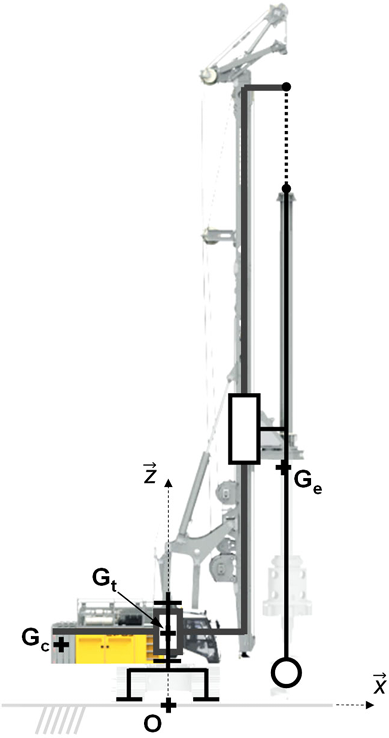
\includegraphics[width=\linewidth]{fig_05}
\end{center}

On commence donc par modéliser le contact par des liaisons ponctuelles avec frottement. L'écriture du PFS et l'utilisation du modèle de Coulomb permet de déterminer des conditions géométriques à la limite du coincement. 
(Pour cela, on fait l'hypothèse qu'on est à la limite du glissement en un point (égalité) et dans le cône d'adhérence à l'autre point inégalité.) 

%\newpage
%\ifprof
%
%On note $\vect{F_I} = X_I \vect{x} + Y_I\vect{y}$ et $\vect{F_J} = X_J \vect{x} + Y_J\vect{y}$. De plus $\vect{F}=-F\vect{y}$. On considère le jeu négligeable (mais suffisamment grand pour permettre le basculent de la pièce 2 et donc l'arcboutement. En appliquant le PFS en $A$, on a donc : 
%$\left\{
%\begin{array}{l}
%X_I + X_J = 0 \\
%Y_I + Y_J -F = 0 \\ 
%-eF + \dfrac{\ell}{2}X_J - \dfrac{\ell}{2}X_I + \dfrac{D}{2}Y_J - \dfrac{D}{2}Y_I = 0
%\end{array}
%\right.$
%$
%\Longleftrightarrow
%\left\{
%\begin{array}{l}
%X_I + X_J = 0 \\
%Y_I + Y_J -F = 0 \\ 
%-eF + \dfrac{\ell}{2}\left(X_J - X_I\right) + \dfrac{D}{2}\left(Y_J - Y_I\right) = 0
%\end{array}
%\right.$
%
%On a de plus : 
%$
%\left\{
%\begin{array}{l}
%X_I \leq 0 \text{ et } Y_I \geq 0 \\
%X_J \geq 0 \text{ et } Y_J \geq 0 \\
%|Y_I|\leq f|X_I| \text{ et }  |Y_J|\leq f|X_J| \\
%\end{array}
%\right.$
%$
%\Rightarrow
%\left\{
%\begin{array}{l}
%X_I \leq 0 \text{ et }  Y_I \geq 0 \\
%X_J \geq 0 \text{ et } Y_J \geq 0 \\
%Y_I\leq -fX_I \text{ et } Y_J\leq fX_J \\
%\end{array}
%\right.$
%
%On suppose qu'on est à la limite du glissement au point $I$. On a donc : 
%$
%\left\{
%\begin{array}{l}
%X_I + X_J = 0 \\
%Y_I + Y_J -F = 0 \\ 
%-eF + \dfrac{\ell}{2}\left(X_J - X_I\right) + \dfrac{D}{2}\left(Y_J - Y_I\right) = 0 \\
%Y_I= -fX_I
%\end{array}
%\right.$
%
%$
%\Rightarrow
%\left\{
%\begin{array}{l}
%X_J = -X_I   ** \\
%-fX_I + Y_J -F = 0 \\ 
%-eF + \dfrac{\ell}{2}\left(-X_I - X_I\right) + \dfrac{D}{2}\left(Y_J +fX_I\right) = 0 \\
%Y_I= -fX_I **
%\end{array}
%\right.$
%$
%\Rightarrow
%\left\{
%\begin{array}{l}
%X_J = -X_I   ** \\
%Y_J =F  +fX_I ** \\ 
%-eF + \dfrac{\ell}{2}\left(-2X_I \right) + \dfrac{D}{2}\left(F  +2fX_I \right) = 0 \\
%Y_I= -fX_I **
%\end{array}
%\right.$
%
%$
%\Rightarrow
%\left\{
%\begin{array}{l}
%X_J = -X_I   ** \\
%Y_J =F  +fX_I ** \\ 
%-eF -\ell X_I  + \dfrac{D}{2}F  +fDX_I  = 0 \\
%Y_I= -fX_I **
%\end{array}
%\right.$
%$
%\Rightarrow
%\left\{
%\begin{array}{l}
%X_J = -X_I   ** \\
%Y_J =F  +fX_I ** \\ 
% F \left( -e + \dfrac{D}{2} \right) + X_I\left( -\ell+fD\right)   = 0 \\
%Y_I= -fX_I **
%\end{array}
%\right.$
%
%
%$
%\Rightarrow
%\left\{
%\begin{array}{l}
%X_J = -X_I   ** \\
%Y_J =F  +fX_I ** \\ 
%X_I   =  F \dfrac{ -e + \dfrac{D}{2} }{-\ell+fD}=  F \dfrac{ -e + \dfrac{D}{2} }{-\ell+fD} =  F \dfrac{ -2e + D }{-2\ell+2fD}  \\
%Y_I= -fX_I **
%\end{array}
%\right.$
%
%De plus, on  a $Y_J\leq fX_J$. 
%
%En conséquences, 
%
%$F  +fF \dfrac{ -2e + D }{-2\ell+2fD} \leq -fF \dfrac{ -2e + D }{-2\ell+2fD}$
%$\Rightarrow 1  +f\dfrac{ -2e + D }{-2\ell+2fD} \leq -f \dfrac{ -2e + D }{-2\ell+2fD}$
%$\Rightarrow 1  +2f\dfrac{ -2e + D }{-2\ell+2fD} \leq 0$
%$\Rightarrow \dfrac{ -4ef + 2fD-2\ell+2fD }{-2\ell+2fD} \leq 0$
%$\Rightarrow \dfrac{ -2ef + 2fD-\ell }{-\ell+fD} \leq 0$
%\fi
